\chapter{Dados do sistema}
\label{cha:Dados do sistema}

Para satisfazer os requisitos e os casos de uso, foi necessário modelar os dados disponíveis ao sistema e ao algoritmo.

\section{Modelo Entidade-Relacionamento}

A imagem \ref{fig:diagrama-classes} exibe o diagrama do modelo entidade-relacionamento (ER), que descreve os dados no modelos de entidades (coisas de interesse) e seus relacionamentos. O modelo ER segue a notação do Peter Chen \cite{peter-chen}. 

\begin{figure}[ht]
    \begin{center}
    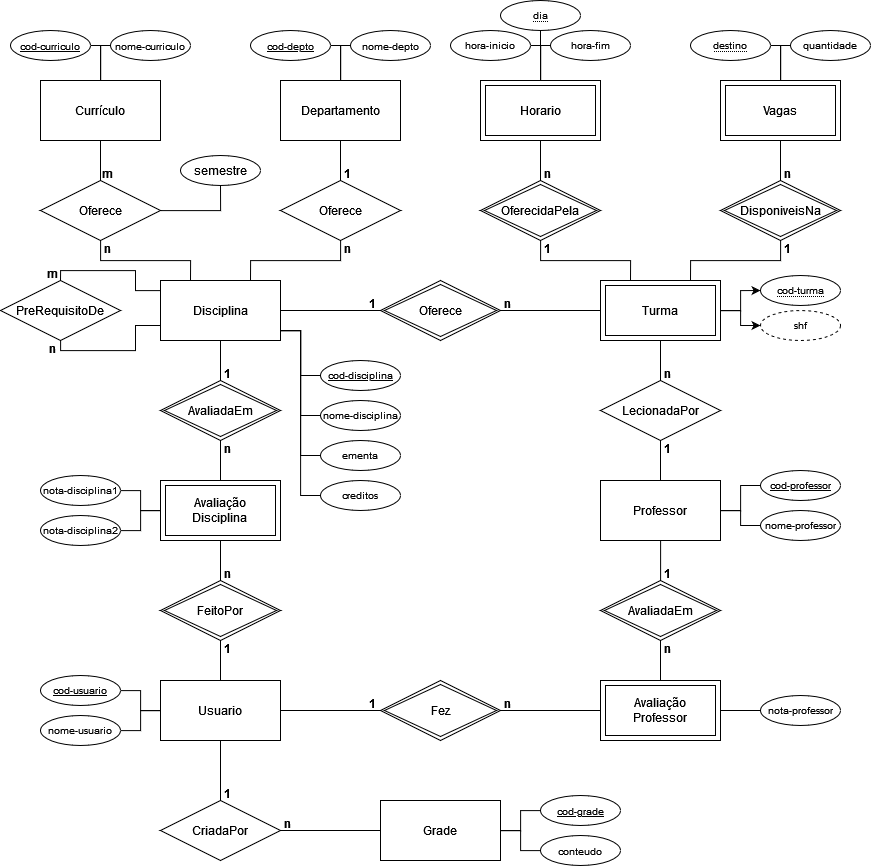
\includegraphics[width=390pt]{figuras/diagrama-er-chen-pdf.png}
    \caption{Diagrama de classes}
    \label{fig:diagrama-classes}
    \end{center}
\end{figure}

\section{Modelo Físico}

A imagem \ref{fig:modelo-fisico} exibe o diagrama físico dos dados com base no modelo ER. Ele representa a estrutura implementada no banco de dados, com suas tabelas e chaves primárias (PK) e chaves estrangeiras (FK).

\begin{figure}[ht]
    \begin{center}
    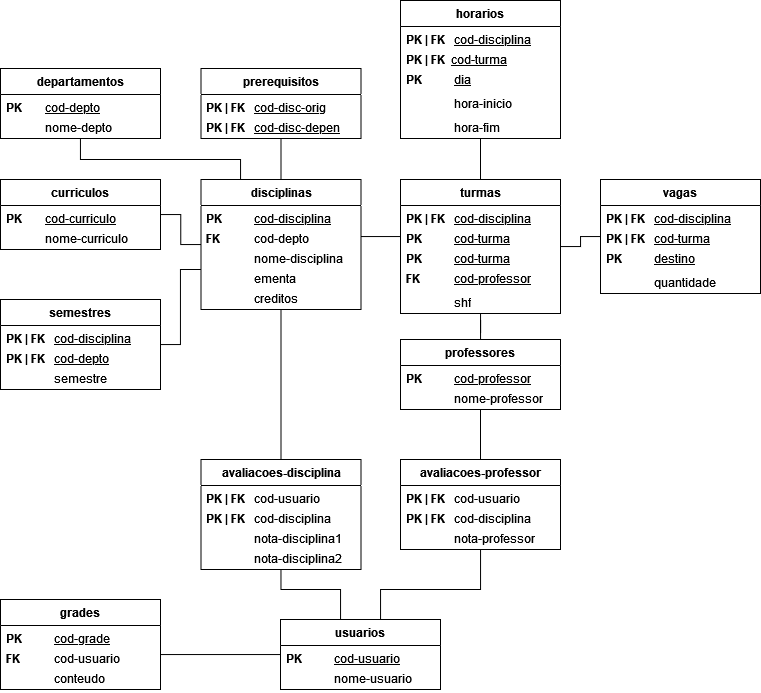
\includegraphics[width=390pt]{figuras/modelo-fisico.png}
    \caption{Modelo físico dos dados}
    \label{fig:modelo-fisico}
    \end{center}
\end{figure}

\section{Dicionario de dados}

aaaaaa a preencher
